\paragraph{Question 1}Le programme linéaire en nombres entiers qui modélise le
  problème du couplage maximum de poids minimum est le suivant.
  (notons $u_{ij}$ les arêtes du graphe)
Notons que $u_{ij} \in \{0, 1\}$ car on prend une arête ou on ne la
prend pas.

\begin{equation}
\begin{cases}
min \sum w_{ij} u_{ij} \\
\forall x_{ij} \in E ~ \sum u_{i' j'} = 1 \\
 x_{i' j'} \in adj(x_{ij}) \cup \{ x_{ij} \} \\
\end{cases}
\end{equation}

En effet, soit $\{ i, j \}$ une arête qui appartient à un couplage
$M$. Par définition, $\Gamma^{-1}(i) $ et $\Gamma^{+1}(j)$
n'appartiennent pas à $M$.

\paragraph{Question 2}
Les équations des contraintes pour le graphe donné par la figure 2
sont les suivantes~:
\begin{equation}
\begin{cases}
u_{ab}+u_{ac}+u_{ae}=1 \\
u_{ab}+u_{bc}+u_{bf}=1 \\
u_{fb}+u_{fd}+u_{fe}=1 \\
u_{ca}+u_{cb}+u_{cd}=1 \\
u_{dc}+u_{df}+u_{de}=1 \\
u_{ef}+u_{ed}+u_{ea}=1 \\
\end{cases}
\end{equation}

\paragraph{Question 3}
Une solution optimale $z(ILP)$ pour le graphe de la figure 2 est un
couplage de taille 3 et de poids $2.\epsilon + M$ ($= 10,2$ en prenant$\epsilon = \dfrac{1}{10}$ et $M=10$), qui peut par
exemple être $\{
ac, bf, de \}$. 

\paragraph{Question 4}
Le programme relaxé consiste à considérer $0 \leq u_{ij} \leq 1$. \\
Nous avons procédé à la modélisation suivante pour le solveur en ligne
de zweigmedia, en prenant $\epsilon = \dfrac{1}{10}$ et $M=10$~:
\begin{lstlisting}
Minimize p = (1/10)uab + (1/10)uac + (1/10)ubc + 10ubf + 10ucd +
(1/10)udf + (1/10)ude + (1/10)ufe + 10uae subject to


uab + uac + uae = 1 
uab + ubc + ubf = 1 
ubf + udf + ufe = 1 
uac + ubc + ucd = 1 
ucd + udf + ude = 1
ufe + ude + uae = 1 

uab >= 0
ubc >= 0
uac >= 0
ubf >= 0
ucd >= 0
uae >= 0
ude >= 0
udf >= 0
ufe >= 0

uab <= 1
ubc <= 1
uac <= 1
ubf <= 1
ucd <= 1
uae <= 1
ude <= 1
udf <= 1
ufe <= 1
\end{lstlisting}

Ce qui nous donne la solution relaxée suivante~:
\begin{lstlisting}
Optimal Solution: p = 0.3; uab = 0.5, uac = 0.5, ubc = 0.5, ubf = 0,
ucd = 0, udf = 0.5, ude = 0.5, ufe = 0.5, uae = 0
\end{lstlisting}
On a donc un couplage de taille $6$ pour un poids de $0,3$.

\paragraph{Question 5}
On remarque une grande différence entre la solution relaxée et la
solution optimale du problème initial, laissant à penser à une
mauvaise modélisation.


La formulation initialement proposée n'est pas pertinente car elle ne
couvre pas tous les cas. Le fait de répondre au problème du couplage
maximum de poids minimum vérifie nos équations, mais la réciproque
n'est pas vrai. On peut ainsi considérer le contre-exemple suivant
dans lequel le couplage obtenu n'est pas maximum~:
\begin{figure}[!ht]
\begin{center}
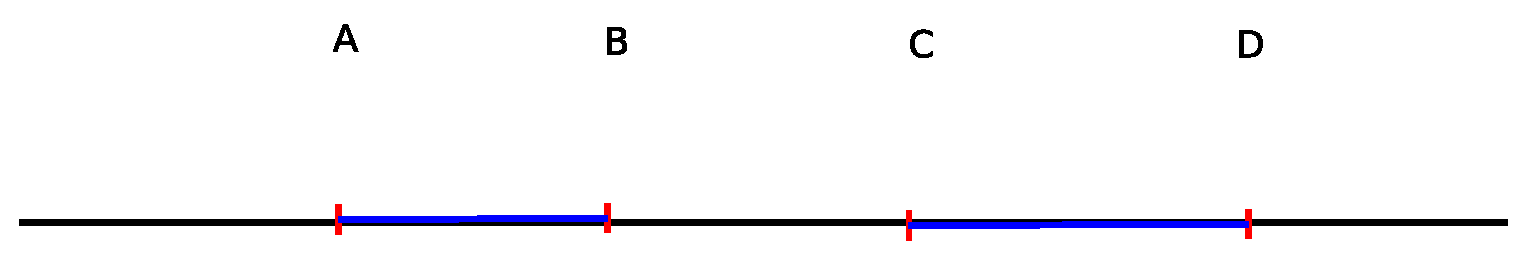
\includegraphics[height=2cm]{exo3.eps}
\end{center}
\caption{Contre exemple pour la formulation proposée à l'exercice 3}
\end{figure}
